% Bake diagram:
%   [ grid bbox enclosing a textured horizontal "ellipsoid" (no cyan fill) ]
%                            │
%                            ▼
%                         [ bake ]
%                            │
%                            ▼
%   [ large square filled with the same noise texture ]
\documentclass[tikz,border=4pt]{standalone}
\usepackage{tikz}
\usepackage{xcolor}
\usepackage{libertine}
\usepackage[libertine]{newtxmath}
\usepackage{amsmath}
\usetikzlibrary{positioning, calc, arrows.meta}

\begin{document}
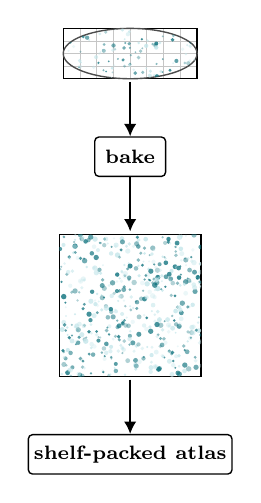
\begin{tikzpicture}[
  font=\sffamily\footnotesize,
  >={Latex[length=4.5pt,width=4.5pt]},
]
\definecolor{cCyan}{HTML}{1F9FAE}

% ============================================================================
% TOP: rectangular bounding box with a grid; horizontal textured ellipsoid
% inside (texture only, no cyan body fill).
% ============================================================================
% Bbox tight around the ellipse: width = 2·eXrT, height = 2·eYrT.
\pgfmathsetmacro{\bboxW}{1.70}
\pgfmathsetmacro{\bboxH}{0.64}
\pgfmathsetmacro{\bboxCx}{0.0}
\pgfmathsetmacro{\bboxCy}{2.50}

\pgfmathsetmacro{\bxL}{\bboxCx - \bboxW/2}
\pgfmathsetmacro{\bxR}{\bboxCx + \bboxW/2}
\pgfmathsetmacro{\byB}{\bboxCy - \bboxH/2}
\pgfmathsetmacro{\byT}{\bboxCy + \bboxH/2}

% Internal grid (8 columns × 4 rows)
\pgfmathsetmacro{\gridDX}{\bboxW/8}
\pgfmathsetmacro{\gridDY}{\bboxH/4}
\foreach \i in {1,...,7} {
  \pgfmathsetmacro{\xpos}{\bxL + \i*\gridDX}
  \draw[gray!45, line width=0.3pt] (\xpos, \byB) -- (\xpos, \byT);
}
\foreach \i in {1,...,3} {
  \pgfmathsetmacro{\ypos}{\byB + \i*\gridDY}
  \draw[gray!45, line width=0.3pt] (\bxL, \ypos) -- (\bxR, \ypos);
}
\draw[black, line width=0.5pt] (\bxL, \byB) rectangle (\bxR, \byT);

% Horizontal textured "ellipsoid" — texture only, no cyan body.
\pgfmathsetmacro{\eXrT}{0.85}
\pgfmathsetmacro{\eYrT}{\eXrT/2.66}
\coordinate (eC) at (\bboxCx, \bboxCy);

\begin{scope}[shift={(eC)}]
  % solid ellipse outline
  \draw[black!70, line width=0.5pt]
    (0,0) ellipse [x radius=\eXrT, y radius=\eYrT];
  \begin{scope}
    \clip (0,0) ellipse [x radius=\eXrT, y radius=\eYrT];
    \pgfmathsetseed{42}
    \foreach \i in {1,...,110} {
      \pgfmathsetmacro{\rx}{(rand)*\eXrT}
      \pgfmathsetmacro{\ry}{(rand)*\eYrT}
      \pgfmathsetmacro{\rs}{0.011 + rnd*0.017}
      \pgfmathsetmacro{\rop}{0.30 + rnd*0.55}
      \pgfmathsetmacro{\rshade}{rnd}
      \ifdim \rshade pt < 0.5pt
        \fill[cCyan!75!black, opacity=\rop] (\rx,\ry) circle (\rs);
      \else
        \fill[cCyan!25!white, opacity=\rop] (\rx,\ry) circle (\rs);
      \fi
    }
  \end{scope}
\end{scope}

% ============================================================================
% bake box (middle)
% ============================================================================
\pgfmathsetmacro{\bakeY}{1.19}     % all three vertical arrows = 0.70
\node[draw=black, line width=0.5pt, rounded corners=1.5pt,
      fill=white, minimum width=9mm, minimum height=5mm,
      align=center, inner sep=2pt,
      font=\rmfamily\bfseries\scriptsize] (bake) at (\bboxCx,\bakeY) {bake};

% arrow: bbox down → bake
\draw[black, line width=0.7pt, ->]
  (\bboxCx,\byB - 0.04) -- (bake.north);

% ============================================================================
% LARGE square: same noise texture, denser, at the bottom
% ============================================================================
\pgfmathsetmacro{\sqSz}{1.80}
\pgfmathsetmacro{\sqCy}{-0.70}
\pgfmathsetmacro{\sqL}{\bboxCx - \sqSz/2}
\pgfmathsetmacro{\sqR}{\bboxCx + \sqSz/2}
\pgfmathsetmacro{\sqB}{\sqCy - \sqSz/2}
\pgfmathsetmacro{\sqT}{\sqCy + \sqSz/2}

% arrow: bake down → square
\draw[black, line width=0.7pt, ->]
  (bake.south) -- (\bboxCx, \sqT + 0.04);

\draw[black, line width=0.5pt] (\sqL,\sqB) rectangle (\sqR,\sqT);
\begin{scope}
  \clip (\sqL,\sqB) rectangle (\sqR,\sqT);
  \pgfmathsetseed{42}
  \foreach \i in {1,...,500} {
    \pgfmathsetmacro{\rx}{\bboxCx + (rand)*\sqSz/2}
    \pgfmathsetmacro{\ry}{\sqCy + (rand)*\sqSz/2}
    \pgfmathsetmacro{\rs}{0.013 + rnd*0.022}
    \pgfmathsetmacro{\rop}{0.30 + rnd*0.55}
    \pgfmathsetmacro{\rshade}{rnd}
    \ifdim \rshade pt < 0.5pt
      \fill[cCyan!75!black, opacity=\rop] (\rx,\ry) circle (\rs);
    \else
      \fill[cCyan!25!white, opacity=\rop] (\rx,\ry) circle (\rs);
    \fi
  }
\end{scope}

% ============================================================================
% "shelf-packed atlas" box, below the noise square
% ============================================================================
\pgfmathsetmacro{\spaY}{-2.59}
\node[draw=black, line width=0.5pt, rounded corners=1.5pt,
      fill=white, minimum width=22mm, minimum height=5mm,
      align=center, inner sep=2pt,
      font=\rmfamily\bfseries\scriptsize] (spa) at (\bboxCx,\spaY)
      {shelf-packed atlas};

\draw[black, line width=0.7pt, ->]
  (\bboxCx,\sqB - 0.04) -- (spa.north);

\end{tikzpicture}
\end{document}
